\documentclass[11pt,aspectratio=169,t]{beamer}
% New shared slide template; deck-specific content remains in main.tex.
\usepackage[T1]{fontenc}
\usepackage{microtype}
\usepackage{helvet}
\usepackage{amsmath,amssymb}
\usepackage{booktabs}
\usepackage{etoolbox}

\usefonttheme[onlymath]{serif}

\definecolor{slideblue}{HTML}{191998}
\setbeamercolor{structure}{fg=slideblue}
\setbeamercolor{block title}{fg=slideblue,bg=slideblue!8}
\setbeamercolor{block body}{fg=black,bg=slideblue!2}
\setbeamerfont{block title}{family=\sffamily,series=\bfseries,size=\normalsize}
\setbeamerfont{block body}{family=\sffamily}
% Compact square blocks: a restrained title strip and a lightly tinted body.
\setbeamertemplate{block begin}{%
  \par\vskip.22em%
  \begin{beamercolorbox}[wd=\linewidth,ht=2.25ex,dp=.55ex,leftskip=.38em,rightskip=.38em]{block title}%
    \usebeamerfont*{block title}\insertblocktitle
  \end{beamercolorbox}%
  \nointerlineskip%
  \begin{beamercolorbox}[wd=\linewidth,leftskip=.38em,rightskip=.38em]{block body}%
    \vskip.28ex\usebeamerfont{block body}%
}
\setbeamertemplate{block end}{%
    \vskip.28ex%
  \end{beamercolorbox}%
  \vskip.22em%
}
\setbeamerfont{title}{series=\bfseries}
\setbeamerfont{frametitle}{series=\bfseries}
\setbeamersize{text margin left=.55cm,text margin right=.55cm}
% Narrow, fixed gutter for every two-column frame.
\newlength{\twocolumngutter}
\setlength{\twocolumngutter}{.18cm}
\newcommand{\tightcolumnwidth}{.49\textwidth}
\newcommand{\mwgscanstart}{\vspace*{-.22cm}}
\setbeamertemplate{navigation symbols}{}
\setbeamertemplate{items}[circle]
% Ordered lists use plain text numerals, without circles or projected icons.
\setbeamertemplate{enumerate item}{\insertenumlabel.}
\setbeamertemplate{enumerate subitem}{\insertenumlabel.\insertsubenumlabel.}
\setbeamertemplate{enumerate subsubitem}{\insertenumlabel.\insertsubenumlabel.\insertsubsubenumlabel.}
\setbeamercolor{enumerate item}{fg=black}
\setbeamercolor{enumerate subitem}{fg=black}
\setbeamercolor{enumerate subsubitem}{fg=black}

\setbeamertemplate{frametitle}{%
  \begin{beamercolorbox}[sep=.6cm,wd=\paperwidth]{frametitle}\usebeamerfont{frametitle}%
  \vbox{}\vskip-1ex\hspace{-.045cm}\strut\insertframetitle\strut\par\vskip-1ex
  \end{beamercolorbox}\vskip.155cm}

\makeatletter
\apptocmd{\itemize}{\ifnum\@itemdepth=1\itemsep8.5pt\else\itemsep9.3pt\vspace{3.4pt}\fi}{}{}
\makeatother
\pdfstringdefDisableCommands{\def\textsuperscript#1{#1}\def\hspace#1{}\def\\{, }}

% Minimal, consistent statement boxes for authored material.
\newenvironment{definitionbox}[1][Definition]{\begin{block}{#1}}{\end{block}}
\newenvironment{theorembox}[1][Theorem]{\begin{block}{#1}}{\end{block}}
\newenvironment{propositionbox}[1][Proposition]{\begin{block}{#1}}{\end{block}}
\newenvironment{exercisebox}[1][Exercise]{\begin{block}{#1}}{\end{block}}
\newcommand{\statementitem}[2]{%
  \par\noindent\hangindent=2.2em\hangafter=1%
  \textcolor{slideblue}{\bfseries(#1)}\enspace #2\par}
\newcommand{\statementsubitem}[2]{%
  \par\noindent\hangindent=3.6em\hangafter=1\hspace*{1.35em}%
  \textcolor{slideblue}{(#1)}\enspace #2\par}


\usepackage{hyperref}
\usepackage{tikz}
\usetikzlibrary{arrows.meta,decorations.pathreplacing,patterns}

\newtheorem{proposition}{Proposition}
% Document Title
\title{\textbf{Mathematics Bootcamp}}
\subtitle{Functions, Counting, The Real Numbers}
\author{Miguel Vázquez-Carrero} 
\date{\textbf{September 2025}}

\begin{document}

\begin{frame}
\titlepage
\end{frame}

\begin{frame}{Bartle-Sherbert - Real Analysis}
\begin{columns}[c,onlytextwidth] % fixed narrow gutter
    \column{\tightcolumnwidth}
        \hfill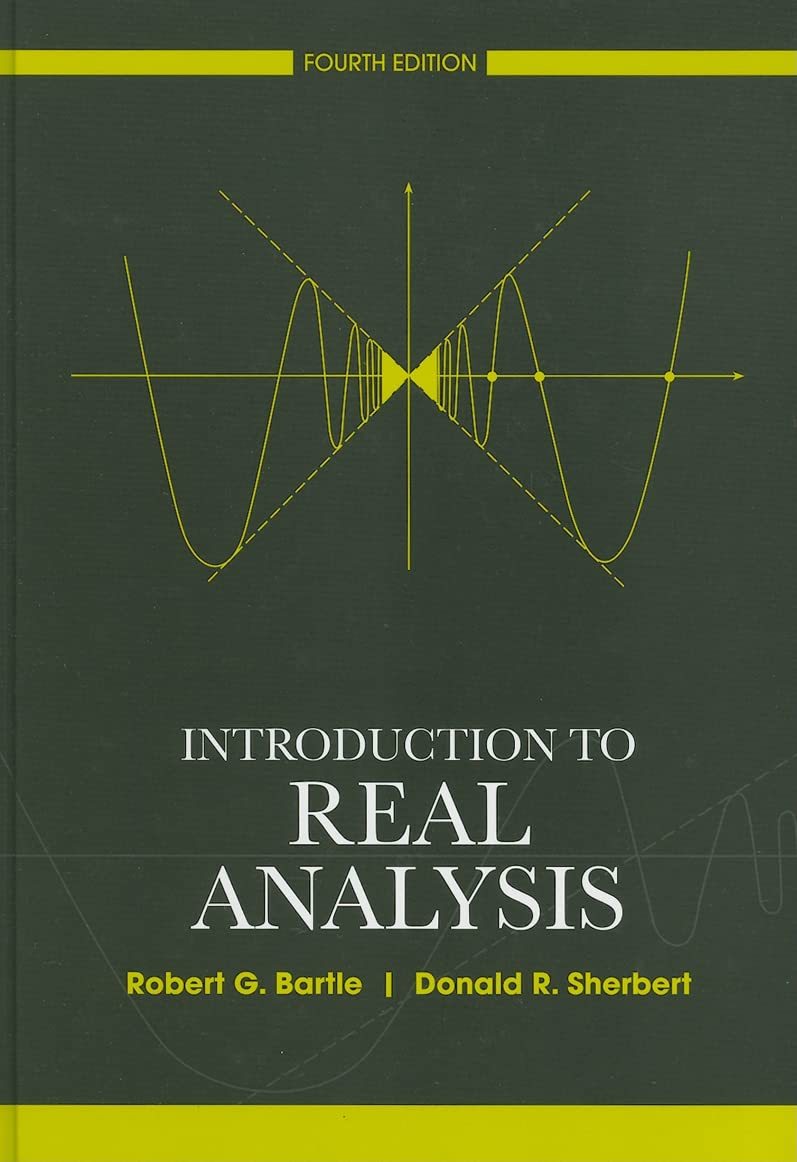
\includegraphics[height=0.77\textheight,keepaspectratio]{bartle-cover.jpg}
    \hspace{\twocolumngutter}
    \column{\tightcolumnwidth}
    \vspace{-2em}
\begin{itemize}
    \item Most of what follows is taken from Bartle-Sherbert.
    \vspace{1em}
    \item My favorite introductory book for Graduate Level Math.
    \begin{itemize}
        \item Careful attention to detail.
        \item Great pedagogical order.
    \end{itemize}
\end{itemize}

\end{columns}
\end{frame}
\begin{frame}{Cartesian Product}
\begin{definitionbox}[1.1.5 Definition]
If $A$ and $B$ are nonempty sets, then the \textbf{Cartesian product} $A\times B$ of $A$
and $B$ is the set of all ordered pairs $(a,b)$ with $a\in A$ and $b\in B$. That is,
\[
  A\times B:=\{(a,b):a\in A,\ b\in B\}.
\]
\end{definitionbox}

For example, if $A:=\{x\in\mathbb{R}:1\leq x\leq2\}$ and
$B:=\{y\in\mathbb{R}:0\leq y\leq1\text{ or }2\leq y\leq3\}$,
then instead of a rectangle, we should have a drawing such as Figure 1.1.3.

\vspace{.08em}
{\centering
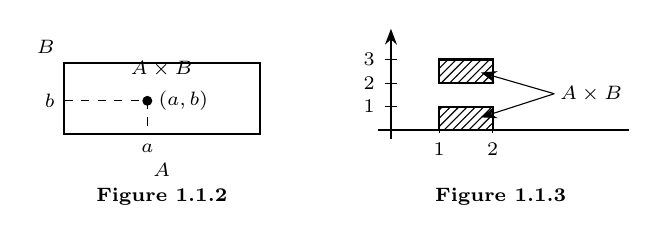
\begin{tikzpicture}[x=.68cm,y=.30cm,>=Stealth,font=\scriptsize]
  % Figure 1.1.2
  \draw[thick] (-6.0,-1.65) rectangle (-2.35,1.35);
  \node at (-4.18,1.08) {$A\times B$};
  \fill (-4.45,-.25) circle (1.8pt);
  \draw[dashed] (-6.0,-.25)--(-4.45,-.25)--(-4.45,-1.65);
  \node[right] at (-4.42,-.25) {$(a,b)$};
  \node[below] at (-4.45,-1.65) {$a$};
  \node[left] at (-6.0,-.25) {$b$};
  \node[above left] at (-6.0,1.35) {$B$};
  \node[below] at (-4.18,-2.48) {$A$};
  \node[below,font=\scriptsize] at (-4.18,-3.52) {\textbf{Figure 1.1.2}};

  % Figure 1.1.3
  \draw[thick,-{Stealth[length=2mm]}] (.1,-1.85)--(.1,2.8);
  \draw[thick] (-.15,-1.5)--(4.55,-1.5);
  \foreach \x in {1,2}{
    \draw (\x,-1.62)--(\x,-1.38);
    \node[below] at (\x,-1.62) {\x};
  }
  \foreach \y in {1,2,3}{
    \draw (-.02,\y-1.5)--(.22,\y-1.5);
    \node[left] at (-.02,\y-1.5) {\y};
  }
  \fill[pattern=north east lines] (1,-1.5) rectangle (2,-.5);
  \draw[thick] (1,-1.5) rectangle (2,-.5);
  \fill[pattern=north east lines] (1,.5) rectangle (2,1.5);
  \draw[thick] (1,.5) rectangle (2,1.5);
  \draw[-{Stealth[length=2mm]}] (3.15,.05)--(1.78,.95);
  \draw[-{Stealth[length=2mm]}] (3.15,.05)--(1.78,-.95);
  \node[right] at (3.08,.05) {$A\times B$};
  \node[below,font=\scriptsize] at (2.15,-3.52) {\textbf{Figure 1.1.3}};
\end{tikzpicture}
\par}
\end{frame}

\begin{frame}{Functions}
\begin{definitionbox}[1.1.6 Definition]
Let $A$ and $B$ be sets. Then a \textbf{function} from $A$ to $B$ is a set $f$ of ordered
pairs in $A\times B$ such that for each $a\in A$ there exists a unique $b\in B$ with
$(a,b)\in f$. (In other words, if $(a,b)\in f$ and $(a,b')\in f$, then $b=b'$.)
\end{definitionbox}

\vspace{.65em}
The set $A$ of first elements of a function $f$ is called the \textbf{domain} of $f$ and is often denoted
by $D(f)$. The set of all second elements in $f$ is called the \textbf{range} of $f$ and is often denoted by
$R(f)$. Note that, although $D(f)=A$, we only have $R(f)\subseteq B$. (See Figure 1.1.4.)

\vspace{.65em}
The essential condition that
\[
  (a,b)\in f\qquad\text{and}\qquad(a,b')\in f
  \qquad\text{implies that}\qquad b=b'
\]
is sometimes called the \emph{vertical line test}. In geometrical terms it says every vertical line
$x=a$ with $a\in A$ intersects the graph of $f$ exactly once.
\end{frame}

\begin{frame}{Functions as Graphs}
 
\begin{itemize}
    \item A function $f$ maps $a$ into \textit{exactly one} $b$: 
    $f(a) = b$ or $a \mapsto b$
\end{itemize}
    
\begin{center}
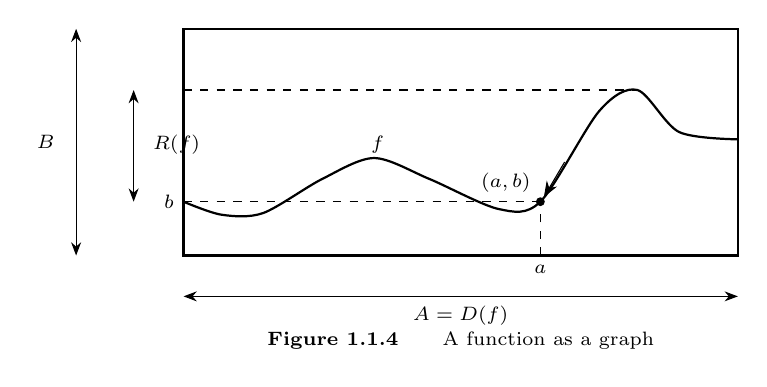
\begin{tikzpicture}[x=.88cm,y=.72cm,>=Stealth,font=\scriptsize]
  \draw[thick] (0,0) rectangle (8,4);
  \draw[thick,smooth]
    plot coordinates {(0,.95) (.55,.72) (1.15,.75) (2.0,1.35) (2.75,1.72)
      (3.55,1.35) (4.55,.82) (5.15,.95) (6.0,2.55) (6.55,2.92)
      (7.15,2.18) (8,2.05)};
  \draw[dashed] (0,.95)--(5.15,.95);
  \draw[dashed] (0,2.92)--(6.55,2.92);
  \draw[dashed] (5.15,0)--(5.15,.95);
  \fill (5.15,.95) circle (1.6pt);
  \node[above left] at (5.15,.95) {$(a,b)$};
  \draw[-{Stealth[length=2mm]}] (5.5,1.65)--(5.2,1.03);
  \node at (2.8,1.95) {$f$};
  \node[left] at (0,.95) {$b$};
  \node[below] at (5.15,0) {$a$};

  \draw[<->] (-1.55,0)--(-1.55,4);
  \node[anchor=east] at (-1.72,2) {$B$};
  \draw[<->] (-.72,.95)--(-.72,2.92);
  \node[anchor=west] at (-.58,1.95) {$R(f)$};
  \draw[<->] (0,-.72)--(8,-.72);
  \node[below] at (4,-.72) {$A=D(f)$};
  \node[below] at (4,-1.18) {\textbf{Figure 1.1.4}\qquad A function as a graph};
\end{tikzpicture}
\end{center}
\end{frame}

\begin{frame}{Functions - Injective and Surjective}
\begin{definitionbox}[1.1.9 Definition]
Let $f:A\to B$ be a function from $A$ to $B$.
\begin{description}
  \item[\textbf{(a)}] The function $f$ is said to be \textbf{injective} (or to be \textbf{one-one})
  if whenever $x_1\neq x_2$, then $f(x_1)\neq f(x_2)$. If $f$ is an injective function,
  we also say that $f$ is an \textbf{injection}.

  \item[\textbf{(b)}] The function $f$ is said to be \textbf{surjective} (or to map $A$ \textbf{onto} $B$)
  if $f(A)=B$; that is, if the range $R(f)=B$. If $f$ is a surjective function, we also say that
  $f$ is a \textbf{surjection}.

  \item[\textbf{(c)}] If $f$ is both injective and surjective, then $f$ is said to be \textbf{bijective}.
  If $f$ is bijective, we also say that $f$ is a \textbf{bijection}.
\end{description}
\end{definitionbox}
\end{frame}

\begin{frame}{Proofs - Injective and Surjective}
\begin{itemize}
  \item In order to prove that a function $f$ is injective, we must establish that:
  \[
    \text{for all }x_1,x_2\text{ in }A,\quad
    \text{if }f(x_1)=f(x_2),\text{ then }x_1=x_2.
  \]
  To do this we assume that $f(x_1)=f(x_2)$ and show that $x_1=x_2$.

  \item To prove that a function $f$ is surjective, we must show that for any $b\in B$
  there exists at least one $x\in A$ such that $f(x)=b$.
\end{itemize}
\end{frame}

\begin{frame}{Cardinality - Finite and Infinite Sets}
\begin{definitionbox}[1.3.1 Definition]
\statementitem{a}{The empty set $\varnothing$ is said to have $0$ \textbf{elements}.}
\statementitem{b}{If $n\in\mathbb{N}$, a set $S$ is said to have $n$ \textbf{elements} if there exists
a bijection from the set $\mathbb{N}_n:=\{1,2,\ldots,n\}$ onto $S$.}
\statementitem{c}{A set $S$ is said to be \textbf{finite} if it is either empty or it has $n$ elements
for some $n\in\mathbb{N}$.}
\statementitem{d}{A set $S$ is said to be \textbf{infinite} if it is not finite.}
\end{definitionbox}

\begin{definitionbox}[1.3.6 Definition]
\statementitem{a}{A set $S$ is said to be \textbf{denumerable} (or \textbf{countably infinite})
if there exists a bijection of $\mathbb{N}$ onto $S$.}
\statementitem{b}{A set $S$ is said to be \textbf{countable} if it is either finite or denumerable.}
\statementitem{c}{A set $S$ is said to be \textbf{uncountable} if it is not countable.}
\end{definitionbox}
\end{frame}


\begin{frame}{Paradoxes from Infinity}
\begin{itemize}

\item Many of our intuitions and even formal notions break when we deal with infinity.

\item For instance, the idea of cardinality:
\begin{itemize}
    \item In finite sets is coherent with number of elements in the set.
    \item In infinite sets it characterizes the size of that infinity.
\end{itemize}

\item In particular, number sets:
\begin{itemize}
\item $\mathbb{N, Z, Q}$ are countably infinite, they share the same cardinality. 
\item However, $\mathbb{R}$ is uncountable, from a bigger size of infinity. \par
See Cantor's Diagonal Argument: \href{https://www.youtube.com/watch?v=YIZd23zGV3M}{Link}.
\end{itemize}

\end{itemize}
\end{frame}





\begin{frame}{The Real Numbers}

\begin{itemize}
\item Most of the functions we use are mappings from (and into) $\mathbb{R}$.
\item There are many ways to construct the Real Numbers.

\item I will take a pragmatic approach to characterize the set.
\begin{itemize}
\item Focus on useful properties for mathematical proofs. 
\item Rely on minimal assumptions.
\end{itemize}
\end{itemize}
    
\end{frame}

\begin{frame}{Field and Order Axioms}

\begin{itemize}
\item Field Axioms characterize how the operations of addition and multiplication behave for elements of the set.

\item Order Axioms characterize how inequalities (e.g.\ $(\mathbb{R},>)$) behave, ensuring that any two field elements are comparable. 

\item Any reasonable foundation will guarantee that the Trichotomy Property holds for all the elements in $\mathbb{R}$.
\end{itemize}

\end{frame}

\begin{frame}{Field and Order Axioms}

\begin{block}{Trichotomy Property.} For any $a, b \in \mathbb{R}$, exactly one of the following holds:
\begin{enumerate}
    \item $a>b$
    \item $a<b$
    \item $a=b$
\end{enumerate}
\end{block}

\begin{block}{Corollary.} For any $a \in \mathbb{R}$, exactly one of the following holds:

\begin{enumerate}
\item $a > 0$ \quad (\text{$a$ is positive}), \qquad
\item $a < 0$ \quad (\text{$a$ is negative}), \qquad
\item $a = 0$
\end{enumerate}
\end{block}

\end{frame}


\begin{frame}{Absolute Value and the Real Line}
\small
\begin{definitionbox}[2.2.1 Definition]
\begin{minipage}[c]{.46\linewidth}
The \textbf{absolute value} of a real number $a$, denoted by $|a|$, is defined by
\end{minipage}\hfill
\begin{minipage}[c]{.49\linewidth}
\[
|a|:=
\begin{cases}
 a,  & \text{if } a>0,\\
 0,  & \text{if } a=0,\\
 -a, & \text{if } a<0.
\end{cases}
\]
\end{minipage}
\end{definitionbox}

\noindent\textbf{The Real Line}\hspace{.55em}\rule{.73\linewidth}{.4pt}

\vspace{.35em}
A convenient and familiar geometric interpretation of the real number system is the real line.
In this interpretation, the absolute value $|a|$ of an element $a$ in $\mathbb{R}$ is regarded as the
distance from $a$ to the origin $0$. More generally, the \textbf{distance} between elements $a$ and $b$
in $\mathbb{R}$ is $|a-b|$. (See Figure 2.2.3.)

\vspace{.2em}
\begin{center}
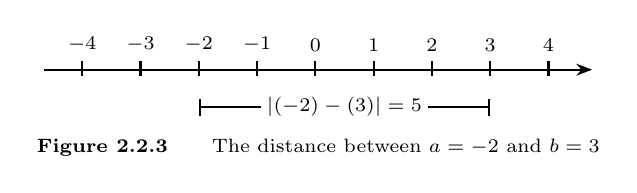
\begin{tikzpicture}[x=.74cm,y=.58cm,>=Stealth,font=\scriptsize]
  \draw[thick,-{Stealth[length=2mm]}] (-4.65,0)--(4.75,0);
  \foreach \x in {-4,-3,...,4}{
    \draw[thick] (\x,-.13)--(\x,.18);
    \node[above] at (\x,.18) {$\x$};
  }
  \draw[|-|,thick] (-2,-.82)--(3,-.82);
  \node[fill=white,inner sep=2pt] at (.5,-.82) {$|(-2)-(3)|=5$};
  \node[below] at (.05,-1.3) {\textbf{Figure 2.2.3}\qquad The distance between $a=-2$ and $b=3$};
\end{tikzpicture}
\end{center}
\end{frame}

\begin{frame}{Distance within the Real Line}
\small
\begin{definitionbox}[2.2.7 Definition]
Let $a\in\mathbb{R}$ and $\varepsilon>0$. Then the $\varepsilon$-\textbf{neighborhood} of $a$ is the set
\[
  V_{\varepsilon}(a):=\{x\in\mathbb{R}:|x-a|<\varepsilon\}.
\]
\end{definitionbox}

For $a\in\mathbb{R}$, the statement that $x$ belongs to $V_{\varepsilon}(a)$ is equivalent to either of the
statements (see Figure 2.2.4)
\[
  -\varepsilon<x-a<\varepsilon
  \quad\Longleftrightarrow\quad
  a-\varepsilon<x<a+\varepsilon.
\]

\begin{center}
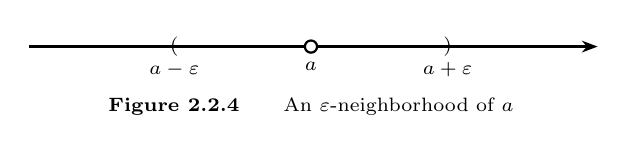
\begin{tikzpicture}[x=1.12cm,y=.65cm,>=Stealth,font=\scriptsize]
  \draw[thick,-{Stealth[length=2mm]}] (-3.2,0)--(3.25,0);
  \draw[very thick] (-1.55,0)--(1.55,0);
  \node at (-1.55,0) {$($};
  \node at (1.55,0) {$)$};
  \draw[fill=white,thick] (0,0) circle (2.2pt);
  \node[below] at (-1.55,-.12) {$a-\varepsilon$};
  \node[below] at (0,-.12) {$a$};
  \node[below] at (1.55,-.12) {$a+\varepsilon$};
  \node[below] at (0,-.82) {\textbf{Figure 2.2.4}\qquad An $\varepsilon$-neighborhood of $a$};
\end{tikzpicture}
\end{center}

\begin{itemize}
    \item How does a Neighborhood look in a 2D, 3D Space?
    \item What about more than 3 Dimensions?
\end{itemize}

\end{frame}

\begin{frame}{Bounds, Suprema, Infima}
\begin{definitionbox}[2.3.1 Definition]
Let $S$ be a nonempty subset of $\mathbb{R}$.
\begin{description}
  \item[\textbf{(a)}] The set $S$ is said to be \textbf{bounded above} if there exists a number
  $u\in\mathbb{R}$ such that $s\leq u$ for all $s\in S$. Each such number $u$ is called an
  \textbf{upper bound} of $S$.

  \item[\textbf{(b)}] The set $S$ is said to be \textbf{bounded below} if there exists a number
  $w\in\mathbb{R}$ such that $w\leq s$ for all $s\in S$. Each such number $w$ is called a
  \textbf{lower bound} of $S$.

  \item[\textbf{(c)}] A set is said to be \textbf{bounded} if it is both bounded above and bounded below.
  A set is said to be \textbf{unbounded} if it is not bounded.
\end{description}
\end{definitionbox}
\end{frame}

\begin{frame}{Bounds, Suprema, Infima}
\small
{\centering
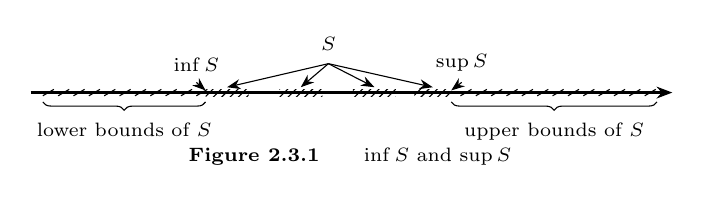
\begin{tikzpicture}[x=.78cm,y=.34cm,>=Stealth,font=\scriptsize]
  \draw[thick,-{Stealth[length=2mm]}] (-5.2,0)--(5.25,0);
  \foreach \x in {-5,-4.75,...,-2.5}{\draw (\x,-.12)--++(.18,.24);}
  \foreach \x in {1.8,2.05,...,5}{\draw (\x,-.12)--++(.18,.24);}
  \fill[pattern=north east lines] (-2.35,-.13) rectangle (-1.65,.13);
  \fill[pattern=north east lines] (-1.15,-.13) rectangle (-.45,.13);
  \fill[pattern=north east lines] (.05,-.13) rectangle (.75,.13);
  \fill[pattern=north east lines] (1.05,-.13) rectangle (1.65,.13);
  \node[above] at (-.35,1.22) {$S$};
  \foreach \x in {-2,-.8,.4,1.35}{\draw[-{Stealth[length=1.7mm]}] (-.35,1.08)--(\x,.2);}
  \node[above] at (-2.5,.42) {$\inf S$};
  \draw[-{Stealth[length=1.7mm]}] (-2.5,.38)--(-2.35,.08);
  \node[above] at (1.82,.42) {$\sup S$};
  \draw[-{Stealth[length=1.7mm]}] (1.82,.38)--(1.65,.08);
  \draw[decorate,decoration={brace,mirror,amplitude=3pt}] (-5,-.35)--(-2.35,-.35)
    node[midway,below=4pt] {lower bounds of $S$};
  \draw[decorate,decoration={brace,mirror,amplitude=3pt}] (1.65,-.35)--(5,-.35)
    node[midway,below=4pt] {upper bounds of $S$};
  \node[below] at (0,-1.72) {\textbf{Figure 2.3.1}\qquad $\inf S$ and $\sup S$};
\end{tikzpicture}
\par}

\begin{definitionbox}[2.3.2 Definition]
Let $S$ be a nonempty subset of $\mathbb{R}$.
\statementitem{a}{If $S$ is bounded above, then a number $u$ is said to be a \textbf{supremum}
(or a \textbf{least upper bound}) of $S$ if it satisfies the conditions:}
\statementsubitem{1}{$u$ is an upper bound of $S$, and}
\statementsubitem{2}{if $v$ is any upper bound of $S$, then $u\leq v$.}
\statementitem{b}{If $S$ is bounded below, then a number $w$ is said to be an \textbf{infimum}
(or a \textbf{greatest lower bound}) of $S$ if it satisfies the conditions:}
\statementsubitem{$1'$}{$w$ is a lower bound of $S$, and}
\statementsubitem{$2'$}{if $t$ is any lower bound of $S$, then $t\leq w$.}
\end{definitionbox}
\end{frame}

\begin{frame}{Completeness Property}
\small
\begin{theorembox}[2.3.6 Completeness Property of $\mathbb{R}$]
\emph{Every nonempty set of real numbers that has an upper bound also has a supremum in $\mathbb{R}$.}
\end{theorembox}

\vspace{.08em}
This property is also called the \textbf{Supremum Property} of $\mathbb{R}$. The analogous property for
infima can be deduced from the Completeness Property as follows. Suppose that $S$ is a nonempty subset
of $\mathbb{R}$ that is bounded below. Then the nonempty set
$\overline{S}:=\{-s:s\in S\}$ is bounded above, and the Supremum Property implies that
$u:=\sup\overline{S}$ exists in $\mathbb{R}$. The reader should verify in detail that $-u$ is the infimum of $S$.

\vspace{.15em}
\begin{itemize}
\setlength{\itemsep}{.18em}
\item This is what distinguishes $\mathbb{R}$ from $\mathbb{Q}$. 
\begin{itemize}
    \setlength{\itemsep}{.08em}
    \item Rationals satisfy field and order axioms but not completeness.
\end{itemize}
\item No Gaps in $\mathbb{R}$. Key implications for Proofs:
\begin{itemize}
\setlength{\itemsep}{.08em}
\item Archimedean Property
\item Density of Rationals
\end{itemize}
\end{itemize}
\end{frame}

\begin{frame}{Key Implications for Proofs}
\small
\begin{theorembox}[Archimedean Property]
\textbf{2.4.3}\quad
\emph{If $x\in\mathbb{R}$, then there exists $n_x\in\mathbb{N}$ such that $x\leq n_x$.}

\vspace{.25em}
\textbf{2.4.6 Corollary}\quad
\emph{If $y>0$, there exists $n_y\in\mathbb{N}$ such that $n_y-1\leq y\leq n_y$.}
\end{theorembox}

\begin{theorembox}[Density Results]
\textbf{2.4.8 Density Theorem}\quad
\emph{If $x$ and $y$ are any real numbers with $x<y$, then there exists a rational number
$r\in\mathbb{Q}$ such that $x<r<y$.}

\vspace{.25em}
\textbf{2.4.9 Corollary}\quad
\emph{If $x$ and $y$ are real numbers with $x<y$, then there exists an irrational number
$z$ such that $x<z<y$.}
\end{theorembox}
\end{frame}

\begin{frame}[t]{Back to Economics - Utility Functions}
\mwgscanstart
{\centering
    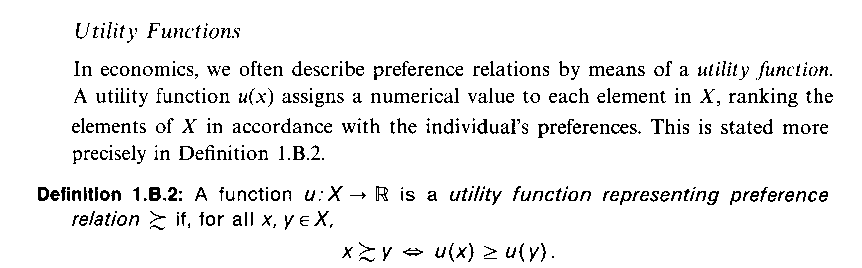
\includegraphics[width=0.96\linewidth,trim=0 0 0 8pt,clip]{mwg-p023-p024-utility.pdf}
\par} 

\end{frame}

\begin{frame}[t]{Utility Functions are Real-Valued Functions}
\par
\mwgscanstart
{\centering
    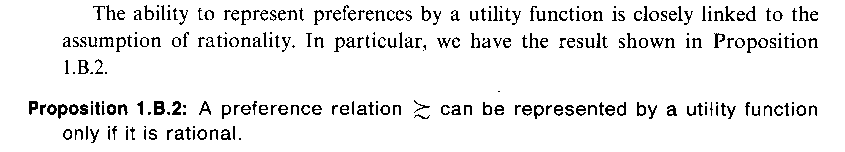
\includegraphics[width=0.96\linewidth,trim=0 0 0 .5pt,clip]{mwg-p024-proposition.pdf}
\par}
\end{frame}
\begin{frame}[t]{Utility Functions}
\par
\mwgscanstart
{\centering
        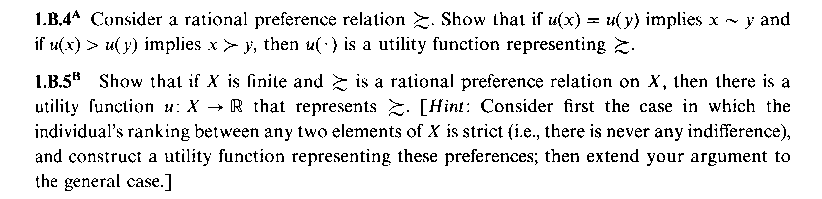
\includegraphics[width=1\linewidth,trim=0 0 0 3pt,clip]{mwg-p030-exercises.pdf}
\par}    
\end{frame}

\end{document}
